\documentclass[a4paper,11pt]{article}
\usepackage{graphicx}
\usepackage{lscape}
\usepackage{capt-of}
\usepackage{fancyhdr}
\usepackage{caption}
\usepackage{subcaption}
\usepackage{tikz}
\usetikzlibrary{arrows.meta}
\usepackage{url}
\usepackage{enumerate}
\usepackage{siunitx}
\usepackage{eurosym}
\usetikzlibrary{quotes,angles,positioning}
\usepackage{standalone}
\usepackage{multirow}
\usepackage{url}
\usepackage{float}
\usepackage{geometry} % to change the page dimensions


\newcommand{\subf}[2]{%
  {\small\begin{tabular}[t]{@{}c@{}}
  #1\\#2
  \end{tabular}}%
}  

\geometry{a4paper} 
\pagestyle{fancy}
\lhead{}
\rhead{}
\renewcommand{\headrulewidth}{0pt}
\setlength\parindent{0pt}
\usepackage{amstext} % for \text
\DeclareRobustCommand{\officialeuro}{%
  \ifmmode\expandafter\text\fi
  {\fontencoding{U}\fontfamily{eurosym}\selectfont e}}
\setlength{\parindent}{5ex}

\begin{document}
\begin{titlepage}

\newcommand{\HRule}{\rule{\linewidth}{0.5mm}} % Defines a new command for the horizontal lines, change thickness here

\center % Center everything on the page
 

%----------------------------------------------------------------------------------------
%	TITLE SECTION
%----------------------------------------------------------------------------------------

\HRule \\[0.4cm]
{ \huge \bfseries Network Software Modelling Assignment 2}\\[0.4cm] % Title of your document
\HRule \\[1.5cm]
 
%----------------------------------------------------------------------------------------
%	AUTHOR SECTION
%----------------------------------------------------------------------------------------

\begin{minipage}{0.4\textwidth}
\begin{flushleft} \large
\emph{Students:}\\
Louis \textsc{Carnec} \\% Your name
Vijay \textsc{Katta}\\
Adedayo \textsc{Adelowokan}  
\end{flushleft}
\end{minipage}
~
\begin{minipage}{0.4\textwidth}
\begin{flushright} \large
\emph{Student \#:} \\
15204934 \\ 15202724 \\15204151 % Supervisor's Name
\end{flushright}
\end{minipage}\\[4cm]

% If you don't want a supervisor, uncomment the two lines below and remove the section above
%\Large \emph{Author:}\\
%John \textsc{Smith}\\[3cm] % Your name

%----------------------------------------------------------------------------------------
%	DATE SECTION
%----------------------------------------------------------------------------------------

{\large \today}\\[3cm] % Date, change the \today to a set date if you want to be precise

%----------------------------------------------------------------------------------------
%	LOGO SECTION
%----------------------------------------------------------------------------------------

%\includegraphics{Logo}\\[1cm] % Include a department/university logo - this will require the graphicx package
 
%----------------------------------------------------------------------------------------

{

	 \vspace{1.5in}\textmd{\textbf{Master of Science (Business Analytics)}}\\
     \large{\textbf{UCD Michael Smurfit Graduate Business School }}\\
      \textmd{\textbf{2016-2017}}\\
 }     
\vfill % Fill the rest of the page with whitespace

\end{titlepage}





\section{Real world phenomenon: Spread of disease through airports network} 


The world is more closely connected than ever before by modern transportation networks. Air, sea and land transportation continues to expand in reach, speed of travel and volume of passengers and goods carried. Pathogens and their vectors can now move further, faster and in greater numbers than ever before \cite{tatem2006global}. Epidemics can occur more easily and the emergence of novel pathogens exacerbates the situation \cite{jones2008global}. Understanding the dispersal behaviour and identifying the outbreak of an epidemic in its preliminary stages enables critical response planning. Network topology properties that surround the debut location can explain much of the early stage variation in the spread of diseases \cite{lawyer2016measuring}.

In this simulation we will model the spread of disease through the US airport network. It is inspired by the work of Yager and Taylor \cite{nicholasyager2014} which model the spread of pathogens through airports around the world using a directed graph. We will extend their work by testing how graphs (subgraphs of the US networks graph with specific properties and Erdos-Renyi graphs with different edge existence probabilities) and initial infection nodes (with different centrality measures) affect the spread of disease through the network.

\section{Describe briefly your choice of graph model and how it corresponds to the real-world phenomenon, e.g. your choice of directed versus undirected edges, edge weights, allowing or disallowing self-loops, etc.}

Our real-world network graph is undirected where nodes represent airports and edges are routes. We used open source data from \url{http://openflights.org}along with population of US cities from \url{https://unstats.un.org/unsd/demographic/products/dyb/City_Page.htm}. Redundant edges and unconnected nodes were removed from the graph. Edge weights were calculates by getting the average population of the two cities connected by edges and normalising for all edges. In creating the graph, only edges connecting airports with the US were added.
The graph created deviates from the real world epidemic scenario. Firstly, exclusively flights within the US are considered. In reality, disease spread through air transport is a world wide phenomenon. In a world wide scenario, we could expect the spread of disease across US nodes to be even quicker as more edges would connect US airport hubs. Secondly, the graph is undirected, this is due to the fact that there is no data for passenger numbers on specific routes. We assume that passenger on routes is proportional to the population of the city which is served by an airport. It is also assumed that routes are bidirectional, to simplify.


\section{With the aid of a diagram, describe the simulation rules, e.g. how agents change state and what causes them to send messages.}

The states of each node/airport are either; susceptible to infection (green), infected (yellow) or dead/closed down (red). All nodes are initially disease free and thus susceptible to infection except from a node which is infected at the beginning, step 0. Once a node is infected, it can infect any of its neighbours with probability related to the edge weight connecting it to its neighbours. In the case where the airport can close down or dies (these terms will be used interchangeably), if the airport has closed down it cannot spread anymore disease, there are no outgoing flights. 


Nodes are coloured based on the status - green is susceptible, yellow is infected and red is removed/dead. The four $K_{2,2}$ graphs in Figures \ref{fig:M1} and \ref{fig:M2} below each one represent the state of nodes in a graph at one time step. Figure \ref{fig:M1} (a), demonstrates the initial state, where node A is infected (yellow) and all other nodes are susceptible (green). In Figure \ref{fig:M1} (b), nodes B and D are infected with probabilities ${\emph{w} _{AB}}$  and ${\emph{w}_{DA}}$ respectively, as they are the neighbours of node A. Figure \ref{fig:M2} (a) shows that all nodes are infected and in (b), the next time step, nodes B and D are red, they are dead/closed indefinitely. 

When a node is dead, it cannot further spread the disease. Therefore, if for example the initial node dies before spreading the disease to a neighbour, for example if it has a low probability of spreading the disease, the spread of the disease will be stopped prematurely.

\begin{figure}[H]
\begin{subfigure}{.3\textwidth}
        \centering
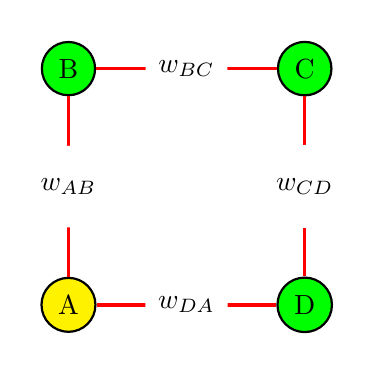
\begin{tikzpicture}
\begin{scope}[every node/.style={circle,thick,draw},local bounding box=aa]
    \node[fill = yellow] (A) at (0,0) {A};
    \node[fill = green] (B) at (0,3) {B};
     \node[fill = green]  (C) at (3,3) {C};
     \node[fill = green]  (D) at (3,0) {D};
\end{scope}

\begin{scope}[>={Stealth[black]},
              every node/.style={fill=white,circle},
              every edge/.style={draw=red,very thick}]
    \path [-] (A) edge node {$w_{AB}$} (B);
    \path [-] (B) edge node {$w_{BC}$} (C);
   \path [-] (C) edge node {$w_{CD}$} (D);
    \path [-] (D) edge node {$w_{DA}$}(A);
\end{scope}
\end{tikzpicture}
\caption{Initial node A infected}
        \label{fig:myfirstsubfig}
    \end{subfigure}%
\begin{subfigure}{.3\textwidth}
        \centering
        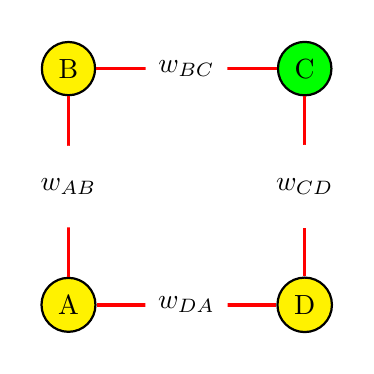
\begin{tikzpicture}
\begin{scope}[every node/.style={circle,thick,draw},shift={(4,0)},local bounding box=bb]
    \node[fill = yellow] (A) at (0,0) {A};
    \node[fill = yellow] (B) at (0,3) {B};
     \node[fill = green]  (C) at (3,3) {C};
     \node[fill = yellow]  (D) at (3,0) {D};
\end{scope}

\begin{scope}[>={Stealth[black]},
              every node/.style={fill=white,circle},
              every edge/.style={draw=red,very thick}]
    \path [-] (A) edge node {$w_{AB}$} (B);
    \path [-] (B) edge node {$w_{BC}$} (C);
   \path [-] (C) edge node {$w_{CD}$} (D);
    \path [-] (D) edge node {$w_{DA}$}(A);
\end{scope}
\end{tikzpicture}
        \caption{B and D infected}
        \label{fig:mysecondsubfig}
    \end{subfigure}
    \caption{Spread of Infection Simulation Rules} \label{fig:M1}
	\end{figure}
\begin{figure}[H]	    
\begin{subfigure}{.3\textwidth}
        \centering
        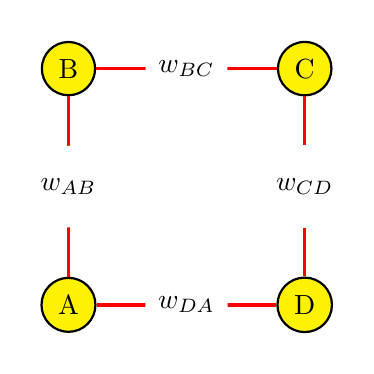
\begin{tikzpicture}
\begin{scope}[every node/.style={circle,thick,draw},shift={(8,0)},local bounding box=bb]
    \node[fill = yellow] (A) at (0,0) {A};
    \node[fill = yellow] (B) at (0,3) {B};
     \node[fill = yellow]  (C) at (3,3) {C};
     \node[fill = yellow]  (D) at (3,0) {D};
\end{scope}

\begin{scope}[>={Stealth[black]},
              every node/.style={fill=white,circle},
              every edge/.style={draw=red,very thick}]
    \path [-] (A) edge node {$w_{AB}$} (B);
    \path [-] (B) edge node {$w_{BC}$} (C);
   \path [-] (C) edge node {$w_{CD}$} (D);
    \path [-] (D) edge node {$w_{DA}$}(A);
\end{scope}
\end{tikzpicture}
        \caption{All nodes infected}
        \label{fig:mysecondsubfig}
    \end{subfigure}
    \begin{subfigure}{.4\textwidth}
        \centering
        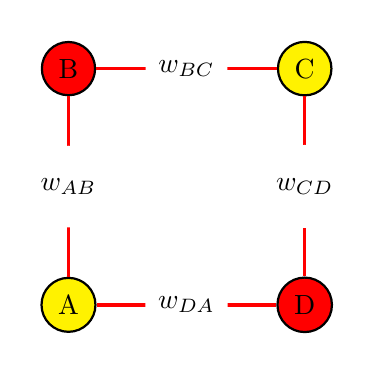
\begin{tikzpicture}
\begin{scope}[every node/.style={circle,thick,draw},shift={(8,0)},local bounding box=bb]
    \node[fill = yellow] (A) at (0,0) {A};
    \node[fill = red] (B) at (0,3) {B};
     \node[fill = yellow]  (C) at (3,3) {C};
     \node[fill = red]  (D) at (3,0) {D};
\end{scope}

\begin{scope}[>={Stealth[black]},
              every node/.style={fill=white,circle},
              every edge/.style={draw=red,very thick}]
    \path [-] (A) edge node {$w_{AB}$} (B);
    \path [-] (B) edge node {$w_{BC}$} (C);
   \path [-] (C) edge node {$w_{CD}$} (D);
    \path [-] (D) edge node {$w_{DA}$}(A);
\end{scope}
\end{tikzpicture}
        \caption{Infected nodes die after n steps}
        \label{fig:mysecondsubfig}
    \end{subfigure}


\caption{Spread of Infection Simulation Rules} \label{fig:M2}
\end{figure}
\section{Program your simulation in Python.}

\section{State one or more simulation properties which you wish to investigate and which graph properties you hypothesise they may depend on.}

\subsection*{Simulation Properties}
We will investigate two main simulation properties; with and without airports being able to close or nodes dying. The hypothesis is that the spread of the disease throughout the network will be slowed down by airport closing as, at each time-step, they cannot spread the disease to neighbours once closed down. \\
Each simulation depends on the probability of being infected at a given timestep ($p_{infection}$) and the time after infection at which the node dies. In both cases $p_{infection} = 0.4$ is multiplied with the edge weight, this gives the 





















\end{document}

